\documentclass[border=3pt]{standalone}
\usepackage{tikz}
\usetikzlibrary{arrows.meta,calc}
\tikzset{pin/.style={-{Stealth[length=5pt]}},
  blk/.style={draw, thick, minimum width=24mm, minimum height=34mm, font=\sffamily\small, align=center}}
\begin{document}
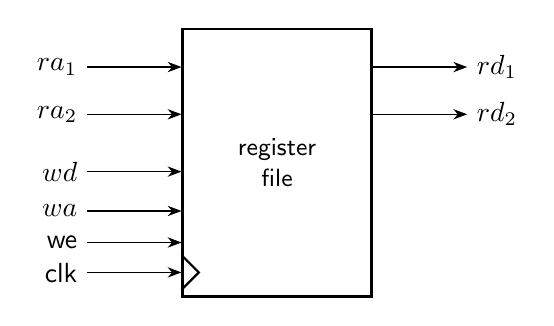
\begin{tikzpicture}[font=\sffamily]
  \node[blk] (rf) {register\\file};
  \draw[thick] ($(rf.south west)+(0,1mm)$) -- ++(2.2mm,2.2mm) -- ++(-2.2mm,2.2mm);
  % read addr in, read data out (two ports)
  \draw[pin] ($(rf.north west)+(-12mm,-5mm)$) node[left]{$ra_1$} -- ($(rf.north west)+(0,-5mm)$);
  \draw[pin] ($(rf.north west)+(-12mm,-11mm)$) node[left]{$ra_2$} -- ($(rf.north west)+(0,-11mm)$);
  \draw[pin] ($(rf.north east)+(0,-5mm)$) -- ++(12mm,0) node[right]{$rd_1$};
  \draw[pin] ($(rf.north east)+(0,-11mm)$) -- ++(12mm,0) node[right]{$rd_2$};
  % write port
  \draw[pin] ($(rf.south west)+(-12mm,11mm)$) node[left]{$wa$} -- ($(rf.south west)+(0,11mm)$);
  \draw[pin] ($(rf.south west)+(-12mm,16mm)$) node[left]{$wd$} -- ($(rf.south west)+(0,16mm)$);
  \draw[pin] ($(rf.south west)+(-12mm,7mm)$) node[left]{we} -- ($(rf.south west)+(0,7mm)$);
  % clk
  \draw[pin] ($(rf.south west)+(-12mm,3.2mm)$) node[left]{clk} -- ($(rf.south west)+(0,3.2mm)$);
\end{tikzpicture}
\end{document}
